\chapter{Заметки}

рассмотрим следующую задачу: у нас есть некоторое количество входов, с произвольным входом. Требуется перераспределить их между тем же количеством выходов, так, чтобы на каждом из них был одинаковый поток.

\

Очевидно, для \underline{произвольного} значения входа, решение единственно:


\vspace{0.5in}

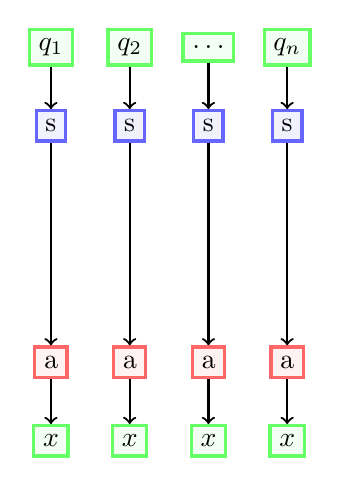
\begin{tikzpicture}[
	s/.style = {rectangle, draw=blue!60,	fill=blue!5,	very thick, minimum size=10},
	a/.style = {rectangle, draw=red!60,		fill=red!5,		very thick, minimum size=10},
	o/.style = {rectangle, draw=green!60,	fill=green!5,	very thick, minimum size=10},
	r/.style = {->, thick, rounded corners=5pt}
	]
	
	
	% === === Nodes === ===
	\node[o]	(in1)	at	(-2, 2)		{$q_1$};
	\node[o]	(in2)	at	(-1, 2)		{$q_2$};
	\node[o]	(ine)	at	(0, 2)		{$\ldots$};
	\node[o]	(inn)	at	(1, 2)		{$q_n$};
	
	\node[s]	(s1)	at	(-2, 1)		{s};
	\node[s]	(s2)	at	(-1, 1)		{s};
	\node[s]	(se)	at	(0, 1)		{s};
	\node[s]	(sn)	at	(1, 1)		{s};
	
	\node[a]	(a1)	at	(-2, -2)	{a};
	\node[a]	(a2)	at	(-1, -2)	{a};
	\node[a]	(ae)	at	(0, -2)		{a};
	\node[a]	(an)	at	(1, -2)		{a};
	
	\node[o]	(out1)	at	(-2, -3)	{$x$};
	\node[o]	(out2)	at	(-1, -3)	{$x$};
	\node[o]	(oute)	at	(0, -3)		{$x$};
	\node[o]	(outn)	at	(1, -3)		{$x$};
	
	
	
	% === === Lines === ===
	\draw[r]	(in1.south)	to	(s1.north);
	\draw[r]	(in2.south)	to	(s2.north);
	\draw[r]	(ine.south)	to	(se.north);
	\draw[r]	(inn.south)	to	(sn.north);
	
	\draw[r]	(a1.south)	to	(out1.north);
	\draw[r]	(a2.south)	to	(out2.north);
	\draw[r]	(ae.south)	to	(oute.north);
	\draw[r]	(an.south)	to	(outn.north);
	
	\draw[r]	(s1.south)	to	(a1.north);
	\draw[r]	(s2.south)	to	(a2.north);
	\draw[r]	(se.south)	to	(ae.north);
	\draw[r]	(sn.south)	to	(an.north);
	
	
\end{tikzpicture}
















\newpage
\thispagestyle{empty}
\mbox{}
\newpage

Входы: 4, 8, 10, 18

Выходы: 5, 8, 12, 15

\

$$
\left[
\begin{matrix}
	5 \\ 8 \\ 15 \\ 12
\end{matrix}
\right]
=
\left[
\begin{matrix}
	\frac12 & 0 & 0 & 0 \\
	0 		& 1 & 0 & 0 \\
	\frac12 & 0 & 1	& \frac13 \\
	0		& 0 & 0 & \frac23 \\
\end{matrix}
\right]
\times
\left[
\begin{matrix}
	10 \\ 8 \\ 4 \\ 18
\end{matrix}
\right]
$$

\

$$
\left[
\begin{matrix}
	10 \\ 8 \\ 4 \\ 18
\end{matrix}
\right]
=
\left[
\begin{matrix}
	1 & 0 & \frac13 & 0 \\
	0 & 1 & 0       & 0 \\
	0 & 0 & \frac23	& \frac13 \\
	0 & 0 & 0       & \frac23 \\
\end{matrix}
\right]
\times
\left[
\begin{matrix}
	5 \\ 8 \\ 15 \\ 12
\end{matrix}
\right]
$$

\

$$
\left[
\begin{matrix}
	\frac12 & 0 & \frac16 & 0 \\
	0 		& 1 & 0       & 0 \\
	\frac12 & 0 & \frac16 & \frac23 \\
	0		& 0 & \frac13 & \frac13 \\
\end{matrix}
\right] \ \equiv \ \left[
\begin{matrix}
	\frac23 & 0 & \frac13 & \frac16 \\
	0 		& 1 & 0       & 0 \\
	0       & 0 & 0       & \frac16 \\
	\frac13	& 0 & \frac23 & \frac13 \\
\end{matrix}
\right] \ \equiv \ \left[
\begin{matrix}
	1 & 0 & 0 & 0 \\
	0 & 1 & 0 & 0 \\
	0 & 0 & 1 & 0 \\
	0 & 0 & 0 & 1 \\
\end{matrix}
\right]
$$





\vspace{0.5in}

$$
\left[
\begin{matrix}
	\alpha\beta + \frac{b-\alpha}{a} - \beta \cdot \frac{b-\alpha}{a} & 
	\alpha \cdot \frac{1-\beta b}{1+a-b} + \frac{b-\alpha}{a} - \frac{b-\alpha}{a} \cdot \frac{1-\beta b}{1 + a - b} \\
	1 - \alpha\beta - \frac{b-\alpha}{a} + \beta \cdot \frac{b-\alpha}{a} & 
	1 - \alpha \cdot \frac{1-\beta b}{1+a-b} - \frac{b-\alpha}{a} + \frac{b-\alpha}{a} \cdot \frac{1-\beta b}{1 + a - b}
\end{matrix}
\right]
\ \equiv \
$$

$$
\ \equiv \
\left[
\begin{matrix}
	\alpha\beta + \frac{1-\beta b}{1 + a - b} - \alpha \cdot \frac{1-\beta b}{1 + a - b} & 
	\beta \cdot \frac{b-\alpha}{a} + \frac{1-\beta b}{1+a-b} - \frac{b-\alpha}{a} \cdot \frac{1 - \beta b}{1 + a - b} \\
	1 - \alpha\beta - \frac{1-\beta b}{1 + a - b} + \alpha \cdot \frac{1-\beta b}{1 + a - b} & 
	1 - \beta \cdot \frac{b-\alpha}{a} - \frac{1-\beta b}{1+a-b} + \frac{b-\alpha}{a} \cdot \frac{1 - \beta b}{1 + a - b}
\end{matrix}
\right]
\ \equiv \
$$

$$
\ \equiv \
\left[
\begin{matrix}
	1 & 0 \\
	0 & 1
\end{matrix}
\right]
$$









































































































































